\documentclass[tikz,border=5mm]{standalone}
\usepackage{tikz}
\usetikzlibrary{arrows.meta, positioning, fit, calc}

\begin{document}
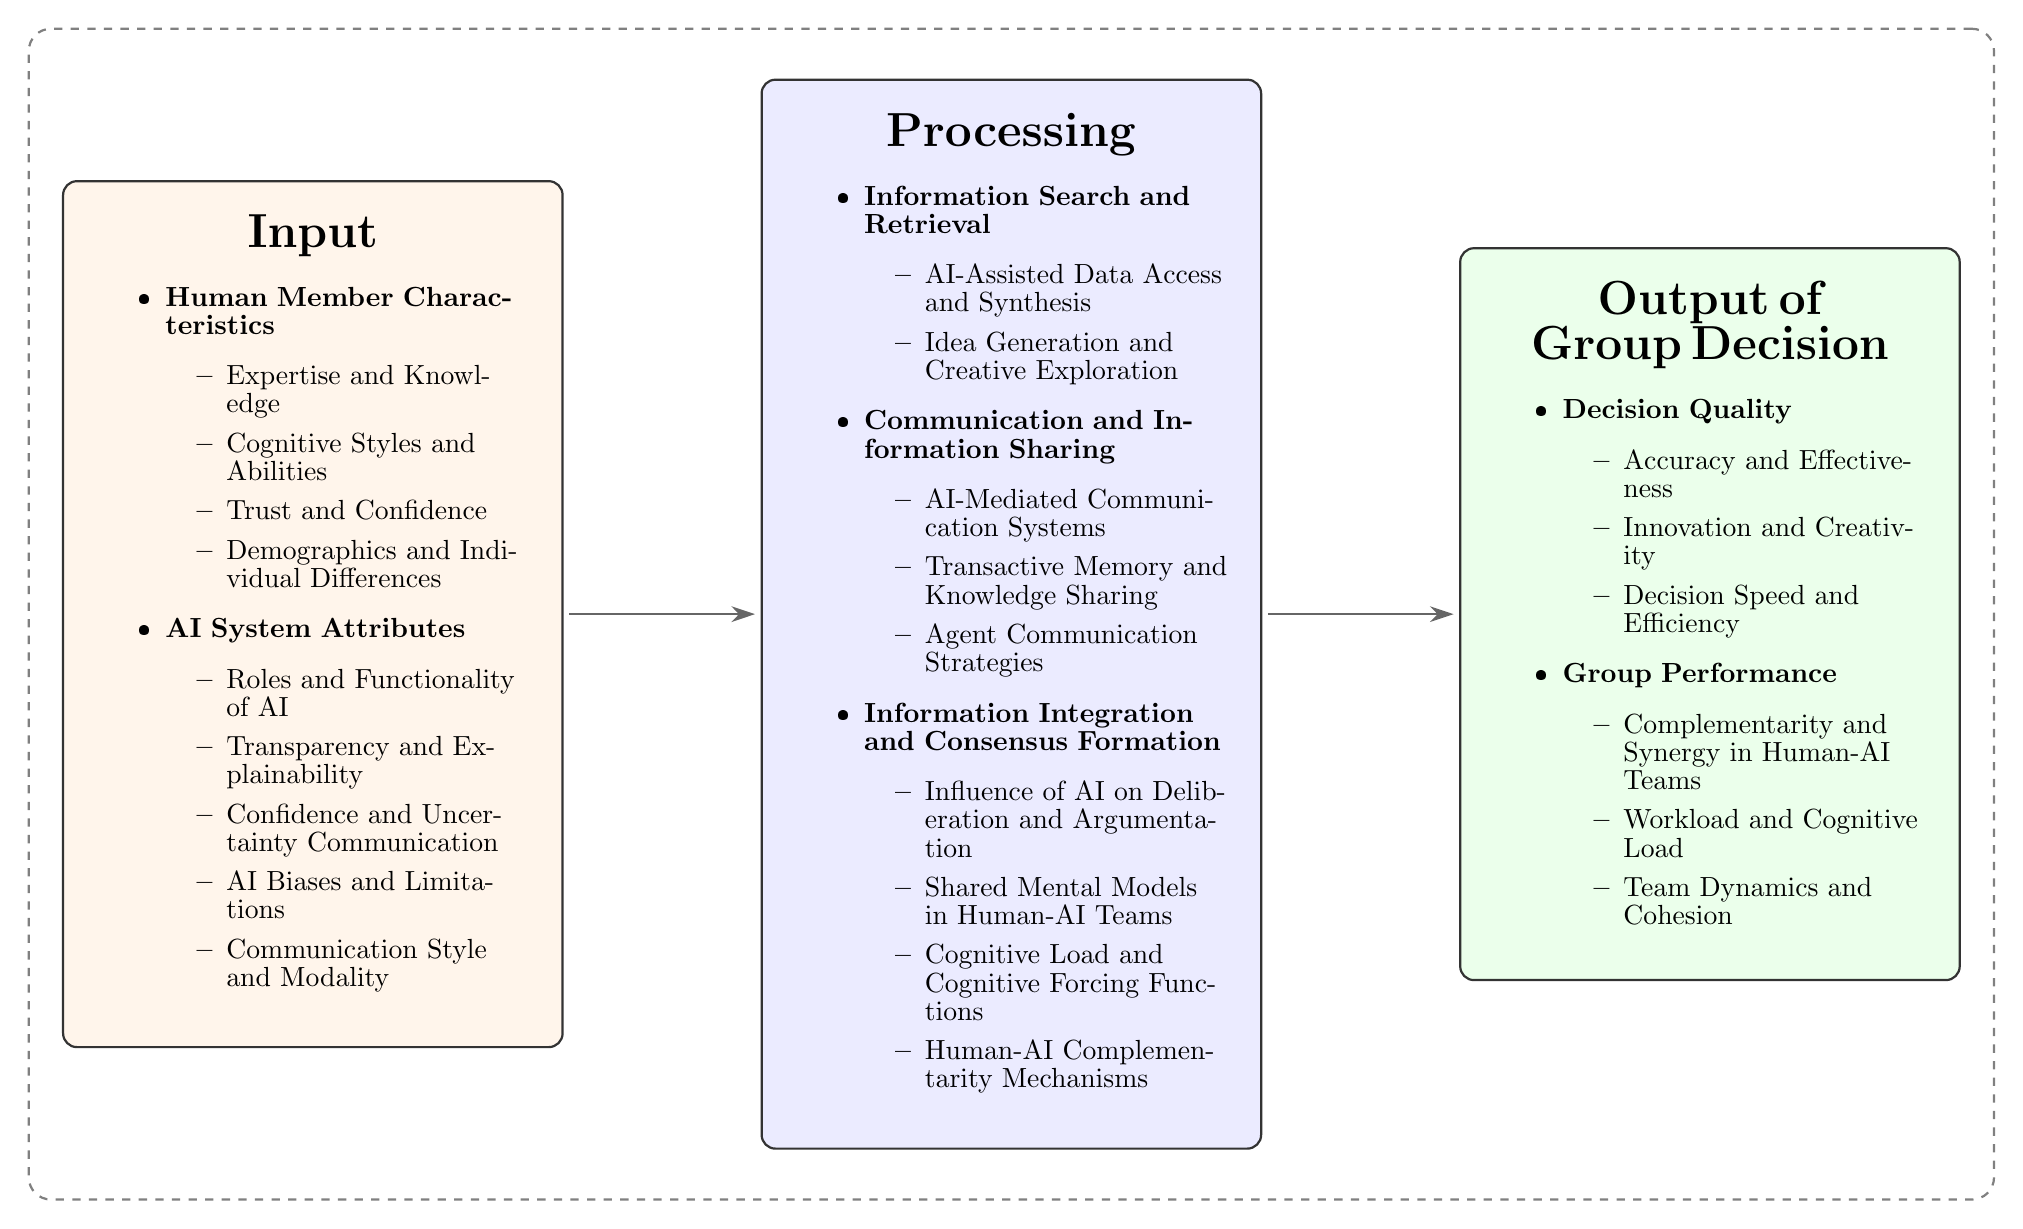
\begin{tikzpicture}[
    every node/.style={font=\normalsize\linespread{0.85}\selectfont},
    box/.style={
        rectangle, 
        rounded corners=5pt,
        draw=black!80,
        thick,
        align=center,
        inner sep=12pt
    },
    inputbox/.style={
        box,
        fill=orange!8,
        text width=5.5cm,
        minimum height=7cm
    },
    processbox/.style={
        box,
        fill=blue!8,
        text width=5.5cm,
        minimum height=7cm
    },
    outputbox/.style={
        box,
        fill=green!8,
        text width=5.5cm,
        minimum height=7cm
    },
    subbox/.style={
        rectangle,
        rounded corners=3pt,
        draw=black!50,
        align=left,
        inner sep=5pt,
        text width=5cm,
        font=\small,
        fill=white,
        text depth=0pt % Added to remove vertical spacing for empty lines
    },
    arrow/.style={
        thick,
        -{Stealth[length=3mm, width=2mm]},
        draw=black!60
    }
]

% Input box
\node[inputbox] (input) {
    \textbf{\LARGE Input} \\[8pt]
    \begin{itemize}
        \item \textbf{Human Member Characteristics}
        \begin{itemize}
            \item Expertise and Knowledge
            \item Cognitive Styles and Abilities
            \item Trust and Confidence
            \item Demographics and Individual Differences
        \end{itemize}
        \item \textbf{AI System Attributes}
        \begin{itemize}
            \item Roles and Functionality of AI
            \item Transparency and Explainability
            \item Confidence and Uncertainty Communication
            \item AI Biases and Limitations
            \item Communication Style and Modality
        \end{itemize}
    \end{itemize}
};

% Processing box
\node[processbox, right=2.5cm of input] (process) {
    \textbf{\LARGE Processing} \\[8pt]
    \begin{itemize}
        \item \textbf{Information Search and Retrieval}
        \begin{itemize}
            \item AI-Assisted Data Access and Synthesis
            \item Idea Generation and Creative Exploration
        \end{itemize}
        \item \textbf{Communication and Information Sharing}
        \begin{itemize}
            \item AI-Mediated Communication Systems
            \item Transactive Memory and Knowledge Sharing
            \item Agent Communication Strategies
        \end{itemize}
        \item \textbf{Information Integration and Consensus Formation}
        \begin{itemize}
            \item Influence of AI on Deliberation and Argumentation
            \item Shared Mental Models in Human-AI Teams
            \item Cognitive Load and Cognitive Forcing Functions
            \item Human-AI Complementarity Mechanisms
        \end{itemize}
    \end{itemize}
};

% Output box
\node[outputbox, right=2.5cm of process] (output) {
    \textbf{\LARGE Output of Group Decision} \\[8pt]
    \begin{itemize}
        \item \textbf{Decision Quality}
        \begin{itemize}
            \item Accuracy and Effectiveness
            \item Innovation and Creativity
            \item Decision Speed and Efficiency
        \end{itemize}
        \item \textbf{Group Performance}
        \begin{itemize}
            \item Complementarity and Synergy in Human-AI Teams
            \item Workload and Cognitive Load
            \item Team Dynamics and Cohesion
        \end{itemize}
        % \item \textbf{Trust and Reliability}
        % \begin{itemize}
        %     \item Calibration of Trust in AI
        %     \item Reliability and Error Management
        %     \item User Satisfaction and Acceptance
        % \end{itemize}
    \end{itemize}
};

% Main flow arrows
\draw[arrow, shorten >=2pt, shorten <=2pt] (input) -- (process);
\draw[arrow, shorten >=2pt, shorten <=2pt] (process) -- (output);

% Framework bounding box
\node[draw=black!50, dashed, thick, rounded corners=8pt, 
       fit=(input) (process) (output),
       inner xsep=12pt, inner ysep=18pt] (frame) {};

\end{tikzpicture}
\end{document}